\documentclass[main.tex]{subfiles}
\begin{document}

\chapter{Statistical Decision Theory: Minimaxity and Admissibility}\label{ch:karar}\chaptermark{Decision Theory}

In earlier chapters we compared estimators by criteria such as unbiasedness, variance and MSE, and tests by level and power. Wald's \cite{wald50} statistical decision theory brings all these criteria into a single framework: a \emph{decision rule\index{decision rule@decision rule}} is a function from the data to an action, and its quality is measured by a \emph{risk function\index{risk function@risk function}} that depends on the true parameter. Estimation, testing and interval construction are special cases of this framework. The trouble is that risk functions usually cross: no rule is best for every $\theta$ (Chapter~\ref{ch:nokta-tahmin}). In this chapter we study the two basic ways of reducing a risk function to a single number: the \emph{Bayes} principle, which minimises the average risk (Chapter~\ref{ch:bayes}), and the \emph{minimax\index{minimax rule@minimax rule}} principle, which minimises the worst case. The bridge between the two principles is the notion of a \emph{least favourable\index{least favourable prior@least favourable prior} prior}. The second theme of the chapter is \emph{admissibility\index{admissibility@admissibility}}, the weakest optimality criterion: here we prove by Blyth\index{blyth s method@Blyth's method}'s method that the normal mean is admissible in one dimension and contrast this with Stein's paradox.

\section{Definitions}

\begin{definition}[Decision Problem and Decision Rule]\label{def:karar-problemi}
A \emph{decision problem} has three components: a parameter space $\Theta$, an \emph{action space} $\mathcal A$ and a loss function\index{loss function@loss function} $L:\Theta\times\mathcal A\to[0,\infty)$. $\X\sim P_\theta$ is observed. A measurable function $\delta:\mathcal X\to\mathcal A$ is called a (non-randomised) \emph{decision rule\index{decision rule@decision rule}}, and $R(\theta,\delta)=\E_\theta L(\theta,\delta(\X))$ its \emph{risk function\index{risk function@risk function}} (Definition~\ref{def:risk}). Examples:
\begin{itemize}
  \item \emph{Point estimation:} $\mathcal A=\Theta$, $L(\theta,a)=(a-\theta)^2$; the risk is the MSE.
  \item \emph{Hypothesis testing:} $\mathcal A=\{0,1\}$ ($1$: reject $H_0$), $L(\theta,a)=\I\{a=1,\theta\in\Theta_0\}+\I\{a=0,\theta\in\Theta_1\}$ (0--1 loss); the risk is the probability of a type I\index{type i and type ii errors@type I and type II errors} error on $\Theta_0$ and of a type II error on $\Theta_1$.
\end{itemize}
\end{definition}

\begin{definition}[Randomised Rule]
A rule that chooses, for each $\x$, a probability distribution $\delta(\cdot\mid\x)$ on $\mathcal A$ is called a \emph{randomised decision rule\index{randomised decision rule@randomised decision rule}}; its risk is $R(\theta,\delta)=\E_\theta\int L(\theta,a)\,\delta(da\mid\X)$. The $\gamma$ in Neyman--Pearson\index{neyman pearson lemma@Neyman--Pearson lemma} tests (Chapter~\ref{ch:neyman-pearson}) is a randomisation. Under a convex loss randomisation brings no gain (Jensen\index{jensen s inequality@Jensen's inequality}'s inequality), but it is needed for tests with discrete data and for finite action spaces.
\end{definition}

\begin{definition}[Minimax Rule]\label{def:minimaks}\index{minimax rule@minimax rule|textbf}
A $\delta^*$ satisfying $\displaystyle\sup_{\theta\in\Theta}R(\theta,\delta^*)=\inf_{\delta}\sup_{\theta\in\Theta}R(\theta,\delta)$ is called a \emph{minimax} rule, and the value on the right the \emph{minimax risk}.
\end{definition}

\begin{definition}[Bayes Risk and Least Favourable Prior]\label{def:en-elverissiz}
For a prior $\pi$, $r(\pi,\delta)=\int R(\theta,\delta)\,\pi(d\theta)$ and $r(\pi)=\inf_\delta r(\pi,\delta)$ (Chapter~\ref{ch:bayes}). A $\pi^*$ that maximises $r(\pi)$, i.e.\ satisfies $r(\pi^*)\ge r(\pi')$ for every $\pi'$, is called a \emph{least favourable\index{least favourable prior@least favourable prior} prior}. Intuitively, it is nature's strategy for choosing the parameter that harms the statistician most.
\end{definition}

\begin{definition}[Equaliser Rule]\index{equaliser rule@equaliser rule|textbf}
A rule whose risk function does not depend on $\theta$, i.e.\ $R(\theta,\delta)=c$ is constant, is called an \emph{equaliser} rule.
\end{definition}

\section{Main Theorems and Proofs}

\begin{theorem}[A Bayes Rule Whose Risk Does Not Exceed Its Bayes Risk Is Minimax]\label{thm:bayes-minimaks}\index{minimax rule@minimax rule}
Let $\delta^\pi$ be a Bayes rule with respect to the prior $\pi$, and suppose
\[
\sup_{\theta\in\Theta}R(\theta,\delta^\pi)\le r(\pi,\delta^\pi) .
\]
Then $\delta^\pi$ is minimax and $\pi$ is least favourable\index{least favourable prior@least favourable prior}.
\end{theorem}
\begin{proof}
For any $\delta$, since the supremum of a function is at least any weighted average of it,
\[
\sup_\theta R(\theta,\delta)\ge\int R(\theta,\delta)\,\pi(d\theta)=r(\pi,\delta)\ge r(\pi,\delta^\pi)\ge\sup_\theta R(\theta,\delta^\pi).
\]
This proves minimaxity. For any $\pi'$, also $r(\pi')\le r(\pi',\delta^\pi)=\int R(\theta,\delta^\pi)\pi'(d\theta)\le\sup_\theta R(\theta,\delta^\pi)\le r(\pi,\delta^\pi)=r(\pi)$.
\end{proof}

\begin{corollary}[An Equaliser Bayes Rule Is Minimax]\label{cor:esitleyici-bayes}\index{equaliser rule@equaliser rule}\index{minimax rule@minimax rule}
If a Bayes rule is an equaliser, it is minimax. More generally, if $\pi(\{\theta:R(\theta,\delta^\pi)=\sup_{\theta'}R(\theta',\delta^\pi)\})=1$, i.e.\ the prior puts mass only on points where the risk is largest, then $\delta^\pi$ is minimax.
\end{corollary}
\begin{proof}
In both cases $r(\pi,\delta^\pi)=\int R(\theta,\delta^\pi)\pi(d\theta)=\sup_\theta R(\theta,\delta^\pi)$; apply Theorem~\ref{thm:bayes-minimaks}.
\end{proof}

\begin{theorem}[The Limiting Bayes Method]\label{thm:limit-bayes}\index{limiting bayes method@limiting Bayes method}
Let $\{\pi_k\}$ be a sequence of priors and $\delta$ a decision rule\index{decision rule@decision rule}. If $\sup_\theta R(\theta,\delta)\le\limsup_{k}r(\pi_k)$, then $\delta$ is minimax.
\end{theorem}
\begin{proof}
For any $\delta'$ and every $k$, $\sup_\theta R(\theta,\delta')\ge r(\pi_k,\delta')\ge r(\pi_k)$. Taking $\limsup$, $\sup_\theta R(\theta,\delta')\ge\limsup_kr(\pi_k)\ge\sup_\theta R(\theta,\delta)$.
\end{proof}

This theorem is the standard way of showing that rules which are not Bayes with respect to any proper prior (for example $\bar X$ in the normal model) are minimax; in that case no least favourable prior exists, but ``in the limit'' it is a flat prior.

\begin{theorem}[A Unique Bayes Rule Is Admissible]\label{thm:bayes-kabul}\index{admissibility@admissibility}
Let $r(\pi)<\infty$ and let $\delta^\pi$ be the unique Bayes rule; i.e.\ every $\delta'$ with $r(\pi,\delta')=r(\pi)$ equals $\delta^\pi$ $P_\theta$-a.s.\ for every $\theta$. Then $\delta^\pi$ is admissible.
\end{theorem}
\begin{proof}
If $\delta'$ dominated $\delta^\pi$, then since $R(\theta,\delta')\le R(\theta,\delta^\pi)$ for every $\theta$, $r(\pi,\delta')\le r(\pi,\delta^\pi)=r(\pi)$, i.e.\ $\delta'$ would also be a Bayes rule. By uniqueness $\delta'=\delta^\pi$ a.s.\ under every $P_\theta$; hence the risk functions\index{risk function@risk function} are equal everywhere, and there is no $\theta$ at which $\delta'$ is strictly better. This is a contradiction.
\end{proof}

\begin{remark}
Under squared loss the Bayes rule is the posterior mean, which is uniquely determined for every $\x$ with $m(\x)>0$. Hence if the marginal distribution $m$ and all the $P_\theta$ have the same null sets (e.g.\ in the binomial model, if $\pi$ is non-degenerate), the uniqueness condition holds. Without uniqueness the result can fail: if $\pi$ puts all its mass on a single point $\theta_0$, there are many Bayes rules that behave arbitrarily away from $\theta_0$.
\end{remark}

\begin{theorem}[An Admissible Equaliser Rule Is Minimax]\label{thm:kabul-esitleyici}\index{equaliser rule@equaliser rule}\index{minimax rule@minimax rule}\index{admissibility@admissibility}
If $\delta$ is admissible and an equaliser ($R(\theta,\delta)=c$), then it is minimax.
\end{theorem}
\begin{proof}
If $\sup_\theta R(\theta,\delta')<c$ for some $\delta'$, then $R(\theta,\delta')<c=R(\theta,\delta)$ for every $\theta$; i.e.\ $\delta'$ would dominate $\delta$. Admissibility rules this out; hence $\sup_\theta R(\theta,\delta')\ge c=\sup_\theta R(\theta,\delta)$ for every $\delta'$.
\end{proof}

\begin{theorem}[Blyth's Method \cite{blyth51}]\label{thm:blyth}\index{blyth s method@Blyth's method}
Let $\Theta\subseteq\R$ be an open interval, and let the risk function of every decision rule be continuous in $\theta$. Let $\delta$ be given. For each $k$ let $\pi_k$ be a measure on $\Theta$ (not necessarily finite) and $\delta_k$ a Bayes rule with respect to it; suppose $r(\pi_k,\delta)<\infty$ and, for every $[a,b]\subset\Theta$ with $a<b$,
\[
\frac{r(\pi_k,\delta)-r(\pi_k,\delta_k)}{\pi_k([a,b])}\to0\qquad(k\to\infty).
\]
Then $\delta$ is admissible.
\end{theorem}
\begin{proof}
Let $\delta'$ dominate $\delta$: $R(\theta,\delta')\le R(\theta,\delta)$ for every $\theta$, and $R(\theta_0,\delta')<R(\theta_0,\delta)-2\varepsilon$ at some $\theta_0$, with $\varepsilon>0$. By continuity of the risks, $R(\theta,\delta)-R(\theta,\delta')>\varepsilon$ on some interval $[a,b]$ containing $\theta_0$. Since $\delta_k$ is Bayes, $r(\pi_k,\delta_k)\le r(\pi_k,\delta')$ and
\[
r(\pi_k,\delta)-r(\pi_k,\delta_k)\ge r(\pi_k,\delta)-r(\pi_k,\delta')=\int\big[R(\theta,\delta)-R(\theta,\delta')\big]\pi_k(d\theta)\ge\varepsilon\,\pi_k([a,b]).
\]
This says that the ratio in the assumption is at least $\varepsilon$ for every $k$; a contradiction.
\end{proof}

\section{Worked Examples}

\begin{example}[Normal Mean: $\bar X$ Is Minimax and (in One Dimension) Admissible]\label{ex:xbar-minimaks}
$X_i\iid\Normal(\theta,\sigma^2)$, $\sigma$ known, squared loss. $R(\theta,\bar X)=\sigma^2/n$ is constant.

\emph{Minimaxity\index{minimax rule@minimax rule}.} For the prior $\pi_k=\Normal(0,k)$ the posterior variance is $(n/\sigma^2+1/k)^{-1}$ (Theorem~\ref{thm:normal-normal}), so the Bayes risk\index{bayes risk@Bayes risk} is $r(\pi_k)=\big(n/\sigma^2+1/k\big)^{-1}\uparrow\sigma^2/n$. By Theorem~\ref{thm:limit-bayes}, $\bar X$ is minimax.

\emph{Admissibility\index{admissibility@admissibility}.} By sufficiency we may work with the single observation $Y=\bar X\sim\Normal(\theta,s^2)$, $s^2=\sigma^2/n$; all risk functions\index{risk function@risk function} are continuous (in an exponential family\index{exponential family@exponential family}, integrals under $\E_\theta$ are continuous functions of $\theta$). Let $\pi_k$ be the (unnormalised) measure with density $e^{-\theta^2/(2k)}$; its total mass is $\sqrt{2\pi k}$. The Bayes rule is again $\delta_k=\frac{k}{k+s^2}Y$, and its Bayes risk with respect to the normalised prior is $\frac{ks^2}{k+s^2}$. Hence
\[
r(\pi_k,Y)-r(\pi_k,\delta_k)=\sqrt{2\pi k}\Big(s^2-\frac{ks^2}{k+s^2}\Big)=\frac{\sqrt{2\pi k}\,s^4}{k+s^2}\to0,
\]
and $\pi_k([a,b])=\int_a^be^{-\theta^2/(2k)}d\theta\to b-a>0$. By Theorem~\ref{thm:blyth}, $\bar X$ is admissible; Theorem~\ref{thm:kabul-esitleyici} gives minimaxity a second time.

\emph{The role of dimension.} In two dimensions $\X$ is also admissible \cite{stein56}, but applying Blyth\index{blyth s method@Blyth's method}'s method requires more carefully chosen sequences of priors; in three or more dimensions, by contrast, $\X$ becomes inadmissible (Stein's paradox, Chapter~\ref{ch:nokta-tahmin}). That is, $\X$ is minimax in every dimension, but for $k\ge3$ there are minimax rules (James--Stein\index{james stein estimator@James--Stein estimator}) that are strictly better.
\end{example}

\begin{example}[The Minimax Estimator for a Binomial Proportion \cite{hodges-lehmann50}]\label{ex:binom-minimaks}
$X\sim\text{Bin}(n,p)$, squared loss. For the $\text{Beta}(a,a)$ prior the Bayes rule is $\delta_a=\frac{X+a}{n+2a}$ (Theorem~\ref{thm:beta-binom}). The risk of a rule of the form $cX+d$ is
\[
R(p,cX+d)=c^2np(1-p)+\big((cn-1)p+d\big)^2 .
\]
For $c=\frac1{n+2a}$, $d=\frac a{n+2a}$, the coefficient of $p^2$ is $-c^2n+(cn-1)^2$ and that of $p$ is $c^2n+2d(cn-1)$. Since $cn-1=-2ac$ and $d=ac$, these coefficients are $c^2(4a^2-n)$ and $c^2(n-4a^2)$ respectively; choosing $a=\sqrt n/2$ makes both vanish. The risk is then constant:
\[
R\Big(p,\frac{X+\sqrt n/2}{n+\sqrt n}\Big)=d^2=\frac{1}{4(1+\sqrt n)^2}.
\]
Being an equaliser\index{equaliser rule@equaliser rule} Bayes rule (Corollary~\ref{cor:esitleyici-bayes}), it is minimax, and $\text{Beta}(\sqrt n/2,\sqrt n/2)$ is the least favourable\index{least favourable prior@least favourable prior} prior. The maximum risk of the MLE, $\frac1{4n}$, exceeds the minimax risk; but the minimax rule is better only when $p$ is near $1/2$: the inequality $p(1-p)/n>\frac1{4(1+\sqrt n)^2}$ means $|p-\tfrac12|<\tfrac12\sqrt{1-n/(1+\sqrt n)^2}$. As $n$ grows this interval shrinks, and the minimax rule shrinks needlessly towards $1/2$.
\end{example}

\begin{example}[Tests Are Decision Rules]\label{ex:test-karar}
$\Theta=\{\theta_0,\theta_1\}$, 0--1 loss and the prior $\pi=(\pi_0,\pi_1)$. The posterior expected loss is $\P(\theta_0\mid\x)$ for the decision to reject $H_0$ and $\P(\theta_1\mid\x)$ for the decision to accept. The Bayes rule chooses the smaller:
\[
\delta^\pi(\x)=1\iff\pi_1f(\x;\theta_1)>\pi_0f(\x;\theta_0)\iff\frac{f(\x;\theta_1)}{f(\x;\theta_0)}>\frac{\pi_0}{\pi_1}.
\]
This is a Neyman--Pearson\index{neyman pearson lemma@Neyman--Pearson lemma} test whose threshold is the prior odds (Theorem~\ref{thm:neyman-pearson}). The Bayes risk is $\pi_0\alpha+\pi_1\beta$, a weighted sum of the two error types. By Corollary~\ref{cor:esitleyici-bayes}, the minimax test is the NP test that equalises the two error probabilities ($\alpha=\beta$); with discrete data this equality can be achieved only by randomisation (Section~\ref{sec:risk-kumesi}).
\end{example}

\begin{example}[A Constant Estimator Can Be Admissible]\label{ex:sabit-kabul}
$X\sim\Normal(\theta,1)$, squared loss and $\delta\equiv3$. Since $R(3,\delta)=0$, if some $\delta'$ dominated it we would have $R(3,\delta')=0$, i.e.\ $\delta'(X)=3$ $P_3$-a.s. Since all normal distributions have the same null sets, $\delta'=3$ a.s.\ under every $P_\theta$, and the risks are equal. Hence $\delta\equiv3$ is admissible: admissibility is a necessary, but far from sufficient, condition for being ``good''.
\end{example}

\section{Computational Applications}

\subsection{Risk Curves for a Binomial Proportion}
We compute the exact risk functions\index{risk function@risk function} of the three rules of Example~\ref{ex:binom-minimaks} for $n=16$: the MLE, the Bayes rule for the uniform prior (Laplace's rule) and the minimax\index{minimax rule@minimax rule} rule.

\pycode{code/ch20/c20_1_binomial_risk_curves.py}
\begin{lstlisting}[style=output]
n = 16 | minimax risk (theory) 1/(4(1+sqrt n)^2) = 0.010000
Risk of the minimax rule: min = 0.010000, max = 0.010000  (equaliser)
Maximum risks: MLE = 0.015625 | Laplace = 0.012346 | minimax = 0.010000
Minimax rule better than MLE: p in (0.203, 0.797)  (theory: 0.2, 0.8)
Bayes risks under the uniform prior: MLE = 0.010417 | Laplace = 0.009259 | minimax = 0.010000
\end{lstlisting}

\begin{figure}[h]
\centering
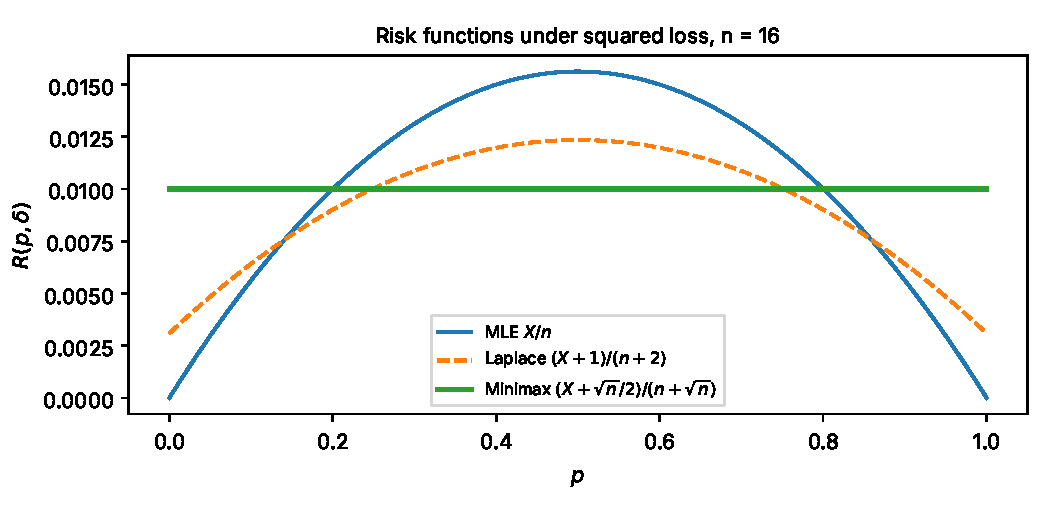
\includegraphics[width=0.85\textwidth]{figures/karar_binom_risk.pdf}
\caption{Risk functions of three estimators under squared loss for $n=16$. The risk of the minimax rule is constant and below the maximum risk of the other two rules; but as $p$ approaches the ends, both other rules are better than it.}
\end{figure}

The output confirms the theory exactly: the risk of the minimax rule is $1/(4\cdot5^2)=0.01$ independently of $p$, and it is better than the MLE only on the interval $p\in(0.2,\,0.8)$. Under the uniform prior the rule with the smallest average risk is Laplace's rule; this is because it is the Bayes rule for this prior. No rule dominates the other two: the choice depends on how we summarise the risk (worst case or average).

\subsection{The Risk Set in a Two-Point Problem}\label{sec:risk-kumesi}
$X\sim\text{Bin}(5,\theta)$, $\theta\in\{0.3,\,0.6\}$ and 0--1 loss. Every subset of $\{0,\dots,5\}$ defines a non-randomised rule\index{randomised decision rule@randomised decision rule} of the form ``decide $\theta_1$ if $X$ is in this set''; each of the $2^6=64$ rules is a point $(R(\theta_0,\delta),R(\theta_1,\delta))$ in the plane. The risk set\index{risk set@risk set} of the randomised rules is the convex hull of these points. The minimax rule is the point where the lower boundary of the hull meets the diagonal; by Theorem~\ref{thm:bayes-minimaks} it corresponds to the Bayes rule for the prior $\pi^*$ that maximises $r(\pi)=\sum_x\min\{\pi f_0(x),(1-\pi)f_1(x)\}$.

\pycode{code/ch20/c20_2_two_point_risk_set.py}
\begin{lstlisting}[style=output]
Number of non-randomised rules: 64
Smallest max. risk among non-randomised rules = 0.3174
Least favourable prior pi* = 0.4274 | minimax risk = max_pi r(pi) = 0.2515
LR threshold = 0.7464, boundary x = [2], randomisation probability gamma = 0.2863
Minimax rule: R0 = 0.2515, R1 = 0.2515 (equal error probabilities)
\end{lstlisting}

\begin{figure}[h]
\centering
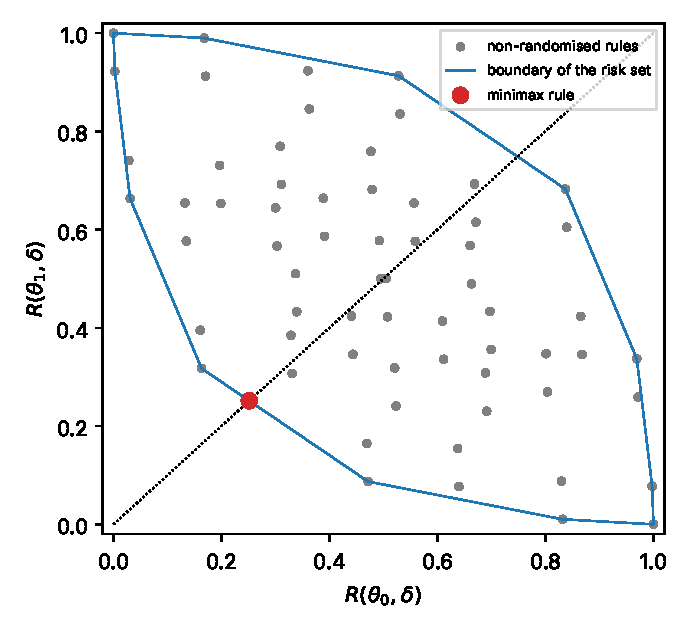
\includegraphics[width=0.5\textwidth]{figures/karar_risk_kumesi.pdf}
\caption{Risk points of the 64 non-randomised rules in the two-point problem and the boundary of the risk set. The red point is the minimax (randomised) rule, where the boundary meets the diagonal.}
\end{figure}

Among non-randomised rules the best maximum risk is $0.3174$; randomisation reduces it to $0.2515$. The minimax rule is the likelihood ratio test\index{likelihood ratio test lrt@likelihood ratio test (LRT)} that decides $\theta_1$ for $X\ge3$ and chooses $\theta_1$ with probability $0.286$ at $X=2$. The threshold equals the odds of the least favourable\index{least favourable prior@least favourable prior} prior ($\pi^*/(1-\pi^*)=0.746$), and since the likelihood ratio at $X=2$ takes exactly this value, the randomisation happens there. The equality of $\max_\pi r(\pi)$ and the minimax risk shows numerically that in this problem the Bayes and minimax approaches meet.

\section{Comments and Notes}

\begin{remark}[A Critique of the Minimax Principle]
The minimax\index{minimax rule@minimax rule} principle is pessimistic: it judges the risk only by its value at the worst $\theta$, and this worst case may not be plausible in reality. In the binomial example the minimax rule is worse than the MLE when $p$ is near the ends, and the region where it is advantageous shrinks as $n$ grows. On the other hand, the minimax risk is a prior-free measure of ``how hard'' a problem is; in nonparametric\index{nonparametric methods@nonparametric methods} statistics and machine learning, optimal rates of convergence (e.g.\ $n^{-4/5}$ in density estimation, Chapter~\ref{ch:parametrik-olmayan}) are expressed in terms of the minimax risk.
\end{remark}

\begin{remark}[Complete Class Theorems]
Wald's \emph{complete class theorems} say that, under suitable regularity conditions\index{regularity conditions@regularity conditions}, every admissible\index{admissibility@admissibility} rule is a Bayes rule or a limit of Bayes rules \cite{wald50,berger85}. In the two-point problem this means that every point on the lower boundary of the risk set\index{risk set@risk set} is Bayes with respect to some prior (Section~\ref{sec:risk-kumesi}). Consequently, a frequentist statistician looking for admissible rules is inevitably led to Bayes rules, while a Bayesian statistician justifies the rule by the chosen prior.
\end{remark}

\begin{remark}[Admissibility and Dimension]
Example~\ref{ex:xbar-minimaks} together with the James--Stein\index{james stein estimator@James--Stein estimator} result of Chapter~\ref{ch:nokta-tahmin} says: in one dimension the natural estimator is both minimax and admissible; in three or more dimensions it remains minimax but is inadmissible. Brown's \cite{brown71} general result ties admissibility to the behaviour of the prior measure at infinity, and thereby to whether a random walk is recurrent; a random walk is recurrent in one and two dimensions, but not in three.
\end{remark}

% --- CHAPTER SUMMARY ---
\section{Chapter Summary}
\begin{summary}
\begin{itemize}
  \item A decision problem consists of a parameter space, an action space and a loss function (Definition~\ref{def:karar-problemi}). Rules are compared by their risk functions; randomisation makes the risk set convex.
  \item The minimax rule minimises the maximum risk (Definition~\ref{def:minimaks}). If the risk of a Bayes rule nowhere exceeds its Bayes risk, the rule is minimax and the prior least favourable (Theorem~\ref{thm:bayes-minimaks}). Bayes rules with constant risk (equalisers) are therefore minimax (Corollary~\ref{cor:esitleyici-bayes}).
  \item When there is no proper prior, the limiting Bayes method with sequences of priors is used (Theorem~\ref{thm:limit-bayes}). For the normal mean, $\bar X$ turns out to be minimax in this way.
  \item A unique Bayes rule is admissible (Theorem~\ref{thm:bayes-kabul}). An admissible equaliser rule is minimax (Theorem~\ref{thm:kabul-esitleyici}). Blyth's method (Theorem~\ref{thm:blyth}) proves admissibility with sequences of priors.
  \item For a binomial proportion the minimax estimator is $(X+\sqrt n/2)/(n+\sqrt n)$, with constant risk. It beats the MLE only when $p$ is near $1/2$: the minimax criterion is a cautious choice geared to the worst case.
\end{itemize}
\end{summary}
% --- END OF CHAPTER SUMMARY ---

\paragraph{Further reading.} \cite{berger85}, \cite[Chapters~4--5]{lehmann-casella}, \cite[Section~7.3.4]{casella}; for the historical foundation, \cite{wald50}.

\section{Exercises}

\begin{exercise}\label{exr:20-1}
Let $X_1,\dots,X_n\iid\text{Poisson}(\lambda)$ with the weighted squared loss $L(\lambda,a)=(a-\lambda)^2/\lambda$. Show that $\bar X$ is an equaliser and, using Theorem~\ref{thm:limit-bayes} with the sequence of $\text{Gamma}(1,b)$ (shape--rate) priors, that it is minimax. (Hint: under this loss the Bayes rule is $1/\E[\lambda^{-1}\mid\x]$.)
\hfill\hyperref[coz:20-1]{\footnotesize$\rightarrow$\,Solution}
\end{exercise}

\begin{exercise}\label{exr:20-2}
Take $n=100$ for the minimax rule of Example~\ref{ex:binom-minimaks}. For which values of $p$ does it have smaller risk than the MLE? Compare the Bayes risks under the uniform prior. What does the ratio of the maximum risks of the two rules converge to as $n\to\infty$?
\hfill\hyperref[coz:20-2]{\footnotesize$\rightarrow$\,Solution}
\end{exercise}

\begin{exercise}\label{exr:20-3}
Show that under squared loss a Bayes rule $\delta^\pi$ with $r(\pi,\delta^\pi)<\infty$ cannot be \emph{unbiased} (except in degenerate cases): prove that if $\delta^\pi$ is unbiased then $\E[(\delta^\pi(\X)-\theta)^2]=0$, by conditioning $\E[\theta\,\delta^\pi]$ under the joint distribution in two different ways. Relate this result to why $\bar X$ is not Bayes with respect to any proper prior in the normal model.
\hfill\hyperref[coz:20-3]{\footnotesize$\rightarrow$\,Solution}
\end{exercise}

\begin{exercise}\label{exr:20-4}
In the problem of Section~\ref{sec:risk-kumesi}, find the Bayes rule and the Bayes risk for the prior $\pi=(1/2,1/2)$. Is this rule minimax? Why?
\hfill\hyperref[coz:20-4]{\footnotesize$\rightarrow$\,Solution}
\end{exercise}

\chapterlinks{20}

\end{document}
